%%%%%%%%%%%%%%%%%%%%%%% file rtree.tex %%%%%%%%%%%%%%%%%%%%%%
% Erweiterungen des R-Baums für räumliche Datenbankanfragen %
%%%%%%%%%%%%%%%%%%%%%%%%%%%%%%%%%%%%%%%%%%%%%%%%%%%%%%%%%%%%%


\documentclass[runningheads,a4paper]{llncs}

\usepackage{amssymb}
\setcounter{tocdepth}{2}
\usepackage{graphicx}
\graphicspath{ {./img/} }           % change graphics include path to ./img/

\usepackage[english, ngerman]{babel}
\usepackage[utf8]{inputenc}			    % for working umlaute
\usepackage[T1]{fontenc}            % wichtig für Trennung von Wörtern mit Umlauten
\usepackage{microtype}						  % verbesserter Randausgleich
\usepackage{pdfpages}
\usepackage{lmodern}		%fuer schoenen Text in pdf-Abbildungen

\usepackage{quoting}
\usepackage[
	babel,
	german=quotes,
	threshold=2,										% two lines ore more triggers a blockquote
	thresholdtype=lines
]{csquotes}
% \SetBlockEnvironment{quoting}			% real block quotes
\renewcommand\mkblockquote[4]{\leavevmode\llap{„}#1#2#3“#4}			% block quotes with german quotation marks

% quellen mangement
\usepackage[
	backend=biber,
	natbib=true,								% damit \citep{} etc. verwendet werden können
	style=authoryear-icomp,    	% Zitierstil
	isbn=false,                	% ISBN nicht anzeigen, gleiches geht mit nahezu allen anderen Feldern
	pagetracker=true,          	% ebd. bei wiederholten Angaben (false=ausgeschaltet, page=Seite, spread=Doppelseite, true=automatisch)
	maxbibnames=10,            	% maximale Namen, die im Literaturverzeichnis angezeigt werden
	maxcitenames=2,            	% maximale Namen, die im Text angezeigt werden, ab 2 wird u.a. nach den ersten Autor angezeigt
	autocite=inline,           	% regelt Aussehen für \autocite (inline=\parancite)
	block=space,               	% kleiner horizontaler Platz zwischen den Feldern
	backref=true,              	% Seiten anzeigen, auf denen die Referenz vorkommt
	backrefstyle=three+,       	% fasst Seiten zusammen, z.B. S. 2f, 6ff, 7-10
	date=short									% Datumsformat
]{biblatex}
\setlength{\bibitemsep}{0.6em}     	% Abstand zwischen den Literaturangaben
\setlength{\bibhang}{2em}        		% Einzug nach jeweils erster Zeile
% \renewcommand{\postnotedelim}{\addcolon\addspace}			% Doppelpunkt statt Komma vor der Seitenangabe in der Zitierung
% \DeclareFieldFormat{postnote}{#1}											% Kein einleitendes «S.» vor der Seitenangabe in der Zitierung

\bibliography{_literatur}

\usepackage[]{acronym}																% für Abkürzungen

\usepackage{hyperref}																	% for hyperlink references
\usepackage[ngerman, nameinlink]{cleveref}						% for naming references

\addto\extrasngerman{\def\figureautorefname{Abb.}}		% changes figure reference text to "Abb."

\usepackage{float}							        							% for use of "H" specifier in floats
\usepackage[section]{placeins}          							% keep floats (images, tables, ..) in their place

% change symbols for unordered lists (itemize)
\renewcommand{\labelitemi}{$\bullet$}
\renewcommand{\labelitemii}{$\circ$}


\begin{document}

\mainmatter  % start of an individual contribution

% first the title is needed
\title{Erweiterungen des R-Baums für räumliche Datenbankanfragen}

\subtitle{Der R*-Baum}

% a short form should be given in case it is too long for the running head
% \titlerunning{Verschiebungsalgorithmen für Kartenbeschriftungen}

\author{Patrick Schulz \& Simon Hötten}

% the affiliations are given next; don't give your e-mail address
% unless you accept that it will be published
\institute{Seminar Geodatenbanken \\ Dozent: Prof. Dr.-Ing. Jan-Henrik Haunert \\ Institut für Geoinformatik und Fernerkundung\\ Universität Osnabrück \\ Sommersemester 2015}

%\toctitle{Titel vom Inhaltsverzeichnis}
%\tocauthor{Authors' Instructions}
\maketitle
% Zusammenfassung
%%%%%%%%%%%%%%%%%%%%%%%%%%%%%%%%%%%%%%%%%%%%%%%%%%%%%%%%%%%%%%%%%%%%
% \begin{abstract}
\keywords{Geodatenbanken, R*, Spatial Access, Index, R-Tree}
% \end{abstract}


% Inhaltsverzeichnis
%%%%%%%%%%%%%%%%%%%%%%%%%%%%%%%%%%%%%%%%%%%%%%%%%%%%%%%%%%%%%%%%%%%%
% \tableofcontents
% \newpage


% Dokument
%%%%%%%%%%%%%%%%%%%%%%%%%%%%%%%%%%%%%%%%%%%%%%%%%%%%%%%%%%%%%%%%%%%%
\section{Motivation} % (fold)
\label{sec:intro}

	Herkömmliche eindimensionale Indexstrukturen bieten keine Möglichkeiten, mehrdimensionale räumliche Daten effizient zu durchsuchen. Die Reduzierung auf Punkte, um Objekte mit \ac{PAM} abzufragen, ist mit gewissen Einbußen möglich, aber insbesondere für komplexere Anfragen unzureichend.
	Der 1984 von Guttman entwickelte R-Baum \citep{Guttman:1984} versucht dieses Problem zu lösen, in dem der Index direkt auf den räumlichen Eigenschaften basiert. Mittlerweile existieren unzählige Varianten und Verwandte des R-Baums, dessen Einsatzgebiet weit über die klassische Geoinformatik hinaus geht.

	Eine dieser Varianten ist der R*-Baum, welcher die (teils unbegründeten) Annahmen in der ursprünglichen Veröffentlichung hinterfragt und so die Datenstruktur weiter optimiert. Im Folgenden gehen wir auf die Verfahren und Eigenheiten des regulären R-, als auch des R*-Baums ein, stellen allgemeine Optimierungskriterien auf und schließen mit einem Vergleich.

	Im Prinzip ist der R*-Baum für n-dimensionale Daten geeignet. Diese Arbeit beschränkt sich allerdings auf Geodaten, insbesondere sind alle Beispiele im zwei dimensionalen Raum. Hier liegt auch das Haupteinsatzgebiet von R*-Bäumen. Für höher-dimensionale Daten sind andere Indexstrukturen, wie der X-Baum, zu bevorzugen \citep[vgl.][28-29]{Kriegel:1996}.

% section intro (end)

\section{Prinzipien eines R-Baums} % (fold)
\label{sec:prinzipien_eines_r_baums}

Der R-Baum ist eine räumliche Indexstruktur für die effiziente Bereichsabfragen von Geometrien im zweidimensionalen Raum. Der R-Baum teilt in jeder Ebene seiner Struktur die beinhalteten Geometrien in Partitionen auf. Die Gesamtheit der Geometrien einer Partitionen werden durch minimal umschließende Rechtecke (kurz \acs{MBR}) repräsentiert. 
Innerhalb einer Partition werden die Geoemtrien in weitere Partitionen unterteilt, bis die Anzahl der Geometrien den Schwellwert \acs{M} innerhalb einer Partition nicht mehr überschreitet. Der Vorteil von dieser Strukturierung sorgt dafür, dass bei Bereichabfragen - zB. Was befindet sich in der Umgebung von Polygon p? - nicht zwingend alle 
Geometrien in der Ebene betrachtet werden müssen: Die \Cref{fig:beispiel-r-tree} stellt einen solchen R-Baum dar, wo bei einer Bereichsabfrage im besten Fall nach der ersten Entscheidungsebene die Hälfte des Geometriebestandes nicht mehr betrachtet werden muss. Die Verwendung von achsparallelen \asc{MBR} sorgt für effiziente Verschneidungs-Abfragen. Durch das alleinige Vergleichen der Koordinaten kann ermittelt werden, ob zwei \asc{MBR} sich schneiden oder nicht. Die Geometrien selbst werden ebenfalls durch \asc{MBR} repräsentiert, sind allerdings zur Bewahrung der Übersichtlichkeit in der \Cref{fig:beispiel-r-tree} nicht dargestellt.
\begin{figure}[H]
		\begin{center}
		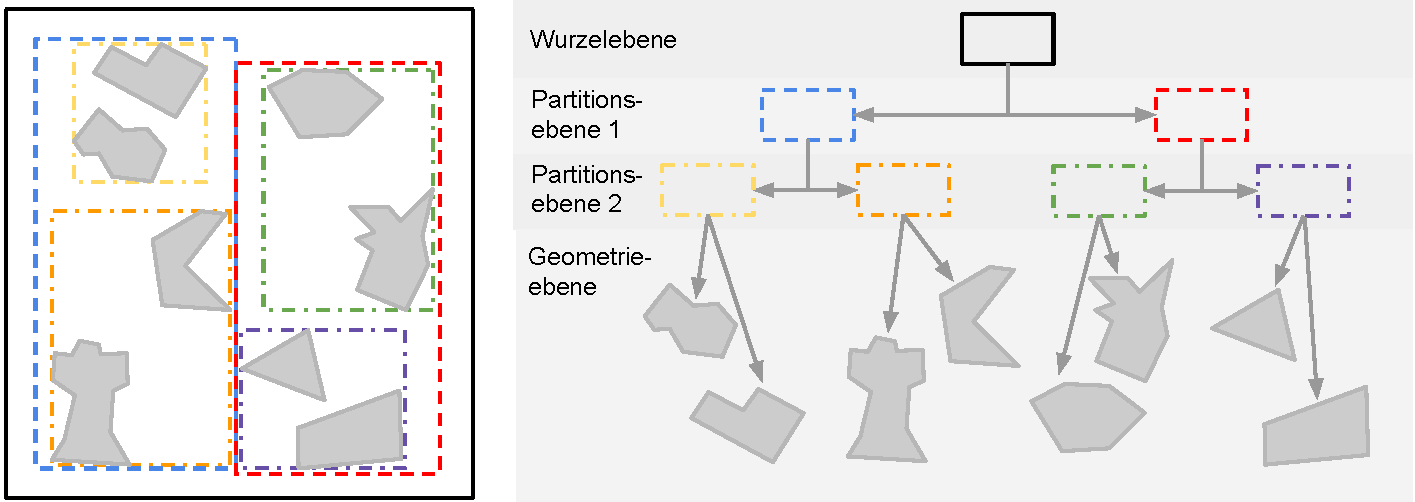
\includegraphics[width=1.0\textwidth ]{001_Beispiel_R-Tree.pdf}
		\caption{Beispiel für einen R-Baum. Links: Verteilung der Polygone und Partitionen im zweidimensionalen Raum. Rechts: Die dazugehörige Baumstruktur. (\acs{M}=3, \acs{m}=2)}
		\label{fig:beispiel-r-tree}
		\end{center}
	\end{figure}
Der Aufbau eines R-Baums verläuft iterativ, wo jedes einzelne Polygon separat nach einem Schema eingefügt wird. Der komplette Prozess des Einfügens lässt sich in zwei Methoden beschreiben, der Author bezeichnet diese Methoden als ChooseSubtree() und QuadraticSplit(). Beide Methoden werden in den nächsten Absätzen beschrieben. Abhängig in welcher Reihenfolge die Polygone in den R-Baum eingesetzt werden kommt es zu verschiedenen Verteilungen innerhalb des R-Baumes. Diese unterschiedlichen Verteilungsmöglichkeiten sind nicht immer ideal und sorgen für weniger effizientere Abfragen, wo durch eine andere Verteilung eine bessere Performance erzielt werden könnte. Die Polygone in der \Cref{fig:beispiel-r-tree} sind im R-Baum zur Veranschaulichung ideal verteilt. Eine Lösung für dieses Problem wird in Kapitel ?(ForcedReInsert)? behandelt und ist Teil der Verbesserungen im R*-Baum.(Beispiel?)

\subsection{ChooseSubTree()}
\label{sec:r-choose-sub}
ChooseSubTree() ist eine rekursive Methode, die für das einzufügende Polygon die paasende Partition in der aktuellen Baum-Ebene zufinden, welches das Polygon daraufhin zugeordnet werden soll. 

\subsection{QuadraticSplit()}
\label{sec:r-split}
QuadraticSplit() wird aufgerufen, sobald innerhalb einer Partition die Anzahl der Geometrien den Wert \asc{M} überschreitet. Wenn der Fall eintritt, muss der Inhalt der überfüllten Partition in zwei neue Partition aufgeteilt werden.  

Verfahren...

Der Grund, wieso die Methode QuadraticSplit() heißt und nicht einfach Split(), liegt daran, dass verschiedene Umsetzungen für die Aufteilung existieren, die eine Unterschiedliche Performance aufweisen. QuadraticSplit() deutet darauf hin, dass die Methode abhängig von der Anzahl Polygone eine quadratische Laufzeit besitzt. Neben dem QuadraticSplit() existieren noch der LinearSplit(), QubicSplit() und der GreenesSplit(). Der LinearSplit() unterscheidet sich vom QuadraticSplit() nur daran, dass dieser die Sortierung der ausstehenden Polygone nur einmal am Anfang durchführt. Dies sorgt zwar für eine bessere Laufzeit, die daraus resultierenden Aufteilungen werden im Vergleich zum QuadraticSplit() allerdings nie besser sein. Der CubicSplit hingegen verspricht, dass nach dem Flächenkriterium die besten Aufteilungen generiert wird auf Kosten der längeren Bearbeitungszeit. Der QuadraticSplit ist somit ein Kompromiss zwischen Effizienz und Qualität.

\subsection{GreenesSplit()}
In einem Paper von "Greenes" wird ein alternatives Verfahren für die bisher bekannten Split-Methoden vorgestellt. Die Idee besteht darin, die Polygone nach der jeweiligen Achse zu sortieren, in der die größte Ausbreitung ermittelt wird. Auf Basis dieser Sortierung hat man nun eine Reihe Splits, aus dem man dann den Favoriten zu ermitteln hat und übernimmt.

% section prinzipien_eines_r_baums (end)

\section{Optimierungskriterien} % (fold)
\label{sec:optimierungskriterien}

	Bei dem herkömmlichen R-Baum wird, sowohl beim Hinzufügen neuer Elemente als auch beim Split, lediglich die Fläche der umschließenden Rechtecke minimiert \citep[vgl.][50-51]{Guttman:1984}. Einige der daraus resultierenden Probleme wurden bereits im vorherigen Abschnitt dargelegt.
	Im Folgenden werden weitere mögliche Optimierungen und ihre Wechselwirkungen aufgeführt. Ein R-Baum muss mit unterschiedlichen Geometrien und Anfragen umgehen können, daher wirken sich einige Kriterien in einigen Situationen stärker aus als andere.

	\subsubsection{Flächenausnutzung maximieren} % (fold)
	\label{ssub:flaechenausnutzung}

	Die Fläche, welche von dem umschließenden Rechteck, aber nicht von den in ihm enthaltenen Rechtecken, überdeckt wird, soll minimiert werden. Es soll also möglichst wenig Platz \enquote{verschwendet} werden. \citep[vgl.][323]{Beckmann:1990}

	% subsubsection flaechenausnutzung (end)

	\subsubsection{Überlappung minimieren} % (fold)
	\label{ssub:ueberlappung_minimieren}

	Die Überlappung der umschließenden Rechtecke soll minimiert werden. Dadurch müssen ebenfalls weniger Pfade im Baum traversiert werden. Liegt ein angefragter Punkt beispielsweise in einer Region, in der sich viele Rechtecke Überschneiden, müssen alle Möglichkeiten weiter verfolgt werden, was zu erhöhtem Rechenaufwand führt.
	
	% subsubsection ueberlappung_minimieren (end)

	\subsubsection{Summe der Kantenlänge minimieren} % (fold)
	\label{ssub:kantenlaenge}

	Die Summe der Kantenlänge der Verzeichnisrechtecke (\emph{\enquote{margin}}) soll möglichst klein sein. Quadrate werden also bevorzugt. Da Quadrate auf den jeweils höheren Ebenen im Baum besser zusammengefasst werden können, reduziert sich so die benötigte Fläche.
	Außerdem profitieren Anfragen mit großen, quadratischen Elementen von dieser Optimierung. \citep[vgl.][323]{Beckmann:1990}
	
	% subsubsection kantenlaenge (end)

	\subsubsection{Speichernutzung maximieren} % (fold)
	\label{ssub:speichernutzung_maximieren}

	Eine geringe Höhe des Baumes wirkt sich positiv auf die Kosten einer Abfrage aus. Das kann durch eine möglichst gleichmaßige Verteilung der Blattknoten erreicht werden. Insbesondere für große Abfragerechtecke ist dies relevant, da hier, auch abgesehen von den ersten drei genannten Optimierungen, mehrere Pfade traversiert werden müssen. \citep[vgl.][323-324]{Beckmann:1990}
	
	% subsubsection speichernutzung_maximieren (end)

	\subsubsection{Wechselwirkungen} % (fold)
	\label{ssub:wechselwirkungen}

	Um die Flächenausnutzung zu maximieren und die Überlappung zu minimieren, bedarf es einer größeren Freiheit bei der Wahl der Formen und der Anzahl an Rechtecken pro Knoten. Die Kriterien stehen also in Konkurrenz mit einer geringen Kantenlänge und hohen Speicherausnutzung. Auf der anderen Seite können quadratischere Rechtecke besser zusammengefasst werden, was sich wiederum positiv auf die Speichernutzung auswirkt. \citep[vgl.][323-324]{Beckmann:1990}
	
	% subsubsection wechselwirkungen (end)

% section optimierungskriterien (end)

\section{Der R*-Baum} % (fold)
\label{sec:rstar_tree}



% section rstar_tree (end)

\section{Fazit} % (fold)
\label{sec:fazit}

	Zunächst lässt sich festhalten, dass der R*-Baum alle vorgestellten Optimierungskriterien berücksichtigt. Das hat einen etwas erhöhten Implementierungsaufwand gegenüber herkömmlichen R-Bumen zur Folge.

	\begin{figure}[H]
		\centering
		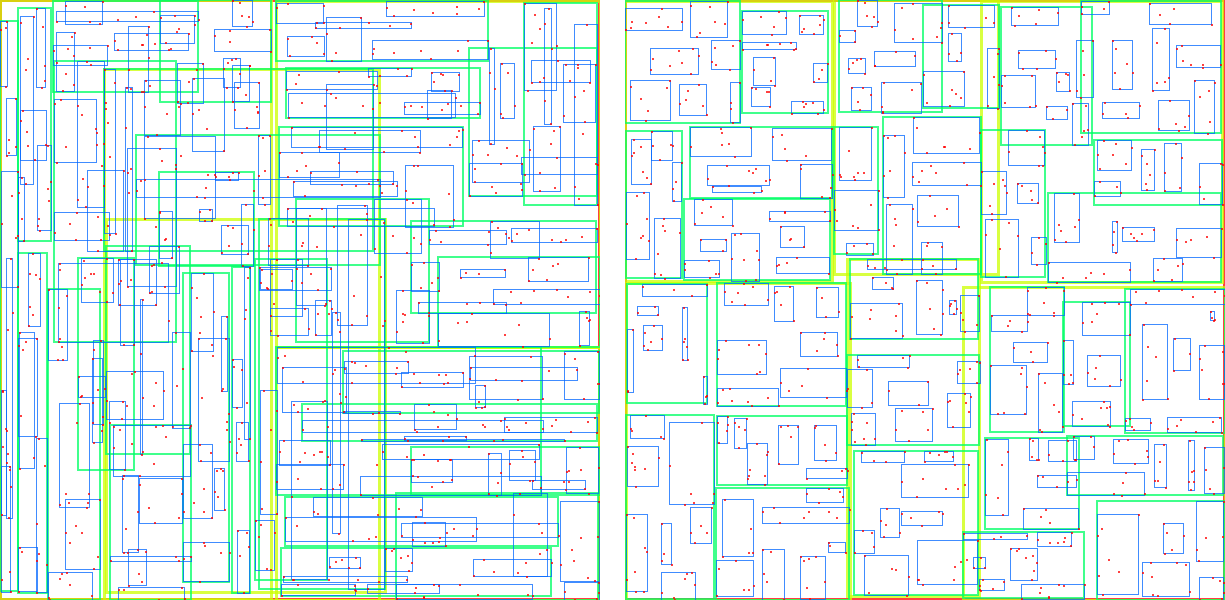
\includegraphics[width=1\textwidth]{vergleich-quad-star.png}
		\caption{Quadratischer- (links) und R*-Split (rechts) im Vergleich. (Bildquelle: \url{https://github.com/davidmoten/rtree})}
		\label{fig:vergleich-quad-star}
	\end{figure}

	Der R*-Baum betreibt sehr hohen Aufwand beim Hinzufügen und Löschen von Elementen, um eine gute Struktur zu bewahren. \Cref{fig:vergleich-quad-star} zeigt den gleichen Datensatz (mit gleicher Einfügereihenfolge), aber unterschiedlichen Split-Verfahren. Das Beispiel zeigt, wie positiv sich der Mehraufwand auswirkt. Mit R*-Split Überschneiden sich die Verzeichnisrechtecke deutlich weniger, was schnellere Abfragen ermöglicht.

	\subsubsection{Benchmarks} % (fold)
	\label{ssub:benchmarks}
	
	% subsubsection benchmarks (end)

	\subsubsection{Weiterentwicklungen} % (fold)
	\label{ssub:weiterentwicklungen}

	Die Effizienz des R*-Baums nimmt ab fünf Dimensionen rapide ab \citep[vgl][29]{Kriegel:2008}. Um auch höher dimensionalen Daten gerecht zu werden, existieren daher zahlreiche Weiterentwicklung. Dazu gehört, wie eingangs erwähnt, der X-Baum, welcher darauf ausgelegt ist auch in höheren Dimensionen Überlappungen zu vermeiden \citep[vgl.]{Kriegel:1996}.
	Andere Indizes bilden Näherungen der tatsächlichen Daten und führen Anfragen zunächst auf diesen aus (\emph{\enquote{Vector Approximation}}, siehe \cite{Gibas:2008} oder \cite{Daoudi:2008}).
	
	% subsubsection weiterentwicklungen (end)

% section fazit (end)



% Anhang
%%%%%%%%%%%%%%%%%%%%%%%%%%%%%%%%%%%%%%%%%%%%%%%%%%%%%%%%%%%%%%%%%%%%
\newpage
\begin{appendix}

	\section*{Anhang}
	\addcontentsline{toc}{section}{Anhang}

	\section*{Abkürzungsverzeichnis} % (fold)
	\label{sub:abbreviations}

		\begin{acronym}[length]
		\acro{m}{Variable: minimale Anzahl der Geometrien in einer Partition}
		\acro{M}{Variable: maximale Anzahl der Geometrien in einer Partition}
		\acro{MBR}{Minimum bounding Rectangle}
	    \acro{SAM}{Spatial access methods}
	    \acro{PAM}{Point access methods}
	  \end{acronym}

	% section abbreviations (end)

	% Abbildungsverzeichnis
	% \listoffigures

	% Literaturverzeichnis
	%%%%%%%%%%%%%%%%%%%%%%%%%%%%%%%%%%%%%%%%%%%%%%%%%%%%%%%%%%%%%%%%%%%%b
	\nocite{*}							% include all bibtex entries from bibliography, even if they are not citied in the document

	\printbibliography

\end{appendix}

\end{document}
